%% Credits of this ams template are with respective people. @Devansh1106 neither own this template nor the credits. 
\documentclass[12pt,reqno]{amsart}

\usepackage{graphicx}

\usepackage{amssymb}
\usepackage{amsthm}
\usepackage{mathrsfs}
\setlength{\parskip}{0.5\baselineskip}%
\setlength{\parindent}{20pt}
\theoremstyle{plain}

\newtheorem*{thm*}{Theorem}
%% this allows for theorems which are not automatically numbered

\renewcommand{\qedsymbol}{$\blacksquare$}
\newtheorem{thm}{Theorem}
\newtheorem{lem}{Lemma}
\newtheorem{exer}{Exercise}
\theoremstyle{definition}
\newtheorem{defn}{Definition}
\newtheorem{eg}{Example}
\newtheorem{rem}{Remark}
\newtheorem*{sol*}{Solution}
\newcommand{\bb}[1]{\mathbb{#1}}
\newcommand{\cal}[1]{\mathcal{#1}}
\usepackage{lineno}
%% The above lines are for formatting.  In general, you will not want to change these.


\title{Deep Learning}
\author{Devansh Tripathi}

\begin{document}

\begin{abstract}
    We shall learn Deep Learning.
\end{abstract}
\maketitle
{\large \part{\centering \\ Shallow Neural Network}} % substitute to chapter or change to amsbook document class

\section{Overflow and Underflow}\label{overflow-and-underflow}

\subsection{Underflow}\label{underflow}

\begin{itemize}
    \item It is the one form of rounding error.
    \item It occurs when numbers near zero are rounded to zero.
    \item Many function can blow up at \(0\) but they maybe defined at some small positive number.
\end{itemize}

\subsection{Overflow}\label{overflow}

\begin{itemize}
    \item It occure when very large number are rounded off as \(\infty\) or \(-\infty\) and for further arithmatic will treat them as \(NaN\).
\end{itemize}

\subsubsection{Avoiding underflow and
overflow}\label{avoiding-underflow-and-overflow}

We should use some trick that stabilize the functions that are present in our algorithm. For example- if we have \(softmax\) function,
\[ \text{softmax}(\bf{x})_i = \frac{\exp(x_i)}{\sum_{j=1}^n \exp(x_j)}\]
then we can use shifting to avoid the any number being too small or too
large. With simple manipulation, it can shown that
\(\text{softmax}(\bf{x}) = \text{softmax}(\bf{x} - c)\) where \(c\) is
\(\max_i x_i\).

Problem will arise when all the entries in the \(\bf x\) are either too
small or too large. But then shifting will make sure at least one
element becomes \(0\) while subtracting the \(\max_ix_i\) namely the
maximum term itself. Then \(\exp{(0)} = 1\) will avoid the underflow and
subtractng \(\max_ix_i\) will make sure all the terms become small to
avoid overflow.

\section{Gradient Descent}\label{gradient-descent}
For \(f(x - \epsilon \text{ sign}(f'(x)))\) is less than \(f(x)\) for
small enough \(\epsilon\). We can thus reduce \(f(x)\) by moving \(x\)
in small steps in the direction opposite to the derivative. This
technique is called \({\it gradient~descent}\). (Cauchy, 1847).

For \(f: {\mathbb R}^n \to {\mathbb R}\),
\({\it directional~derivative}\) in the direction \({\bf u}\) (a unit
vector) is the slope of \(f\) in the direction \(u\).

To minimize \(f\), we need to find the direction in which \(f\)
decreases fastest. So we want the change to be maximum. Since final
value will be less than the initial, the change is negative.

\[ {\bf x}' - {\bf x} = - \epsilon\nabla_{{\bf x}} f({\bf x}) \] where
\({\bf x}'\) is the final value and \({\bf x}\) is the initial value. In
order to maximize RHS, we need to minimize
\(\nabla_{{\bf x}}f({\bf x})\) since \(\epsilon\) is constant (learning
rate).
\begin{align*}
    &= \min\limits_{u, u^\top u=1} \nabla_xf(x) \cdot u \quad \text{(directional derivative)} \\
    &= \min\limits_{u, u^\top u=1} \| u\|_2 \|\nabla_x f(x)\|_2 \cos \theta
\end{align*}
where \(\theta\) is the angle between \(u\) and the gradient. For minimizing this, we need minimal value of \(\cos\theta\) which is \(-1\). Hence, the direction just opposite of gradient is the steepest descent direction. This method is called \({ \it method~of~steepest~descent}\) or \({\it gradient~descent}\).

\textbf{NOTE:} Gradient descent is limited to optimization in continuous
spaces. But general concept of making small moves (that are
approximately the best small move) towards better confiurations can be
generalized towards discrete spaces. TODO: Prove/how this can be
generalized.

\textbf{NOTE}: Ascending an objective function of discrete parameters is
called \({\it hill~climbing}\). (Russel and Norvig, 2003)

\subsection{Line search}\label{line-search}

TODO

\section{Shallow Neural Networks}\label{shallow-neural-networks}
Consider the case with \(D\) hidden units where the \(d\) th hidden unit
is: \[ h_d = a[\theta_{d0} + \theta_{d1}x],\] where \(a[\cdot]\) is the
\emph{activation function} and these are combined linearly to create the
output: \[ y = \phi_0 + \sum\limits_{d=1}^{D} \phi_dh_d.\]

The hidden layer has just \(x\) because there is only one input. In case
of multivariate input, hidden layer will be function of each of the
components of the input.

\begin{figure}[!ht]
    \centering
    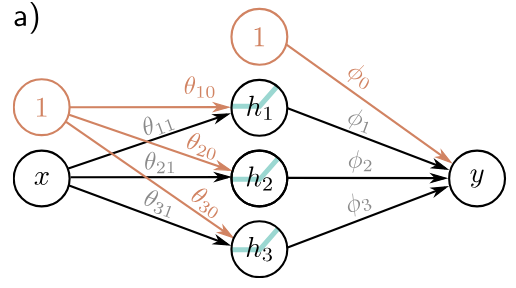
\includegraphics[scale=.36]{../assets/dl/neural_net.png}
    \caption{Neural nets}
\end{figure}

\begin{quote}
{\bf Network Capacity:} The number of hidden units in shallow
network is a measure of network capacity.
\end{quote}
With ReLU activation functions, the output of a network with \(D\) hidden units has atmost \(D\) joints and it is a piecewise linear function with \(D+1\) linear regions.

\begin{quote}
{\bf Universal Approximation Theorem:} This thoerem states that there exists a network with one hidden layer containing finite number of hidden units that can approximate any specified continuous function on a compact subset of $\bb R^n$ to arbitrary accuracy.
\end{quote}

\subsection{Multivariate inputs and
outputs}\label{multivariate-inputs-and-outputs}

\subsubsection{Multivariate Outputs}\label{multivariate-outputs}

To extend the network to multivariate outputs \({\bf y}\), we use
different linear function of the hidden layer for each output. For
example: A network with a scalar input \(x\) and \(4\) hidden layers and
a \(2D\) output \({\bf y} = [y_1, y_2]^\top\) would defined as 

\begin{align*}
    h_1 &= a[\theta_{10} + \theta_{11}x]\\
    h_2 &= a[\theta_{20} + \theta_{21}x]\\
    h_3 &= a[\theta_{30} + \theta_{31}x]\\
    h_4 &= a[\theta_{40} + \theta_{41}x]  
\end{align*}

\begin{figure}[!ht]
    \centering
    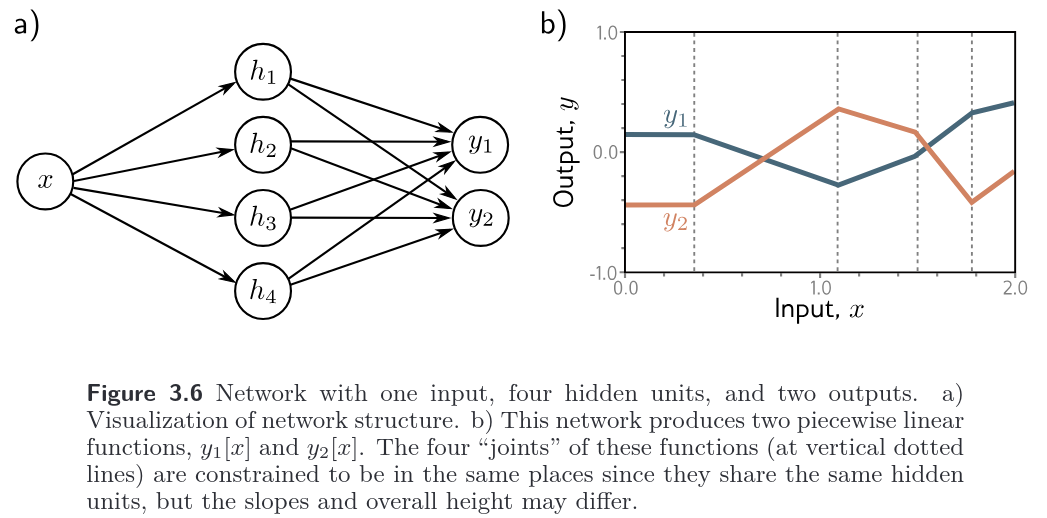
\includegraphics[scale=.34]{../assets/dl/nn2output.png}
    \caption{Neural nets}
\end{figure}
The outputs may look like 
\begin{align*}
    y_1 &= \phi_{10} + \phi_{11}h_1 + \phi_{12}h_2 + \phi_{13}h_3 + \phi_{14}h_4 \\
    y_2 &= \phi_{20} + \phi_{21}h_1 + \phi_{22}h_2 + \phi_{23}h_3 + \phi_{24}h_4 
\end{align*}
Since we are taking the combination of linear functions, the slope of the linear regions can change according to the value \(\phi\)'s {\bf but the location of joints will be same in both outputs}. \(\phi_0\) can cause translation in \(y\) axis.

\begin{exer}
Why the location of joints will not change in the graph of both the outputs which are the linear combination of same hidden layers but for different values of scalar?
\end{exer}
\begin{sol*}
    They are linear combination of same hidden layers (linear functions) with different scalars. When we apply ReLU on them the point of joint gets fixed. Then we create different functions for each output by multiplying the output after ReLU with $\phi$'s which results in change of slope of the line which has non-zero slope. And no change in slope for $0$ slope. (Basically, roots does not change when we multiply slope and intercept by the same number.)
\end{sol*}

\subsubsection{Multivariate Inputs}\label{multivariate-inputs}

In the case of multivariate input \({\bf x}=[x_1, x_2]^\top\), the hidden will be defined as
\[ h_d = a[\theta_{d0} + \theta_{d1}x_1 + \theta_{d2}x_2]\] Then these hidden layers are combined in the usual way of linear combination.

\begin{figure}[!ht]
    \centering
    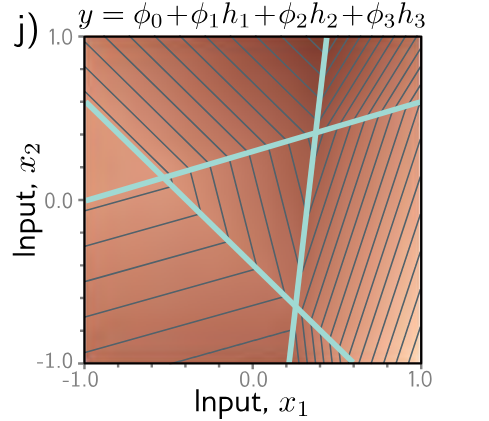
\includegraphics[scale=.34]{../assets/dl/nn2input.png}
    \caption{Convex Region}
\end{figure}
If we had same number of hidden units as input dimensions $D_i$ then we can align each hyperplane with the coordinate axis but in shallow neural networks we usually have more hidden units as compared to input dimensions (hence more than $2^{D_i}$).

\subsection{Shallow Neural Network: General case}
Shallow Neural network ${\bf y = f[x, \boldsymbol{\phi}]}$ maps the multidimensional input ${\bf x} \in \bb R^{D_i}$ to a multidimensional output ${\bf y}\in \bb R^{D_o}$ using ${\bf h} \in \bb R^D$ hidden units. Each hidden unit is computed as:
$$ h_d = a\left[\theta_{d0} + \sum\limits_{i=1}^{D_i}\theta_{di}x_i\right] $$
The final output we get is after linearly combining them:
$$y_j = \phi_{j0} + \sum\limits_{d=1}^{D}\phi_{jd}h_d $$
The model has parameters $\boldsymbol{\phi} = \{\theta_{\bullet, \bullet},\phi_{\bullet, \bullet}\}$. The activation functions permits the model to describe non-linear relations as they itself are non-linear.

With the ReLU activations, the network divides the input space into {\bf convex polytopes} (polygon in higher dimensions) defined by the intersection of hyperplanes computed by joints in the ReLU functions. Each convex polytope contains a different linear function (whichever linear functions are active (nonzero slope) in the region, will contribute to overall polytope). The overall polytope's edge's slope is the summation of the slope of linear functions in the area.

In case of multiple outputs, the polytopes are the same for each output, but the linear function they contain may differ.

\section{Terminology}
\begin{defn}[Pre-activations]
    When we pass data through the network, the values of the inputs to the hidden layer (i.e. before the ReLU functions are applied) are termed as {\it pre-activations}.

    The value at the hidden layer (i.e. after the ReLU functions) are termed as {\it activations}.
\end{defn}
\begin{defn}[Feed forward NN]
    Neural networks in which the connections form an acyclic graph (i.e. graph with no loops, as e.g. in previous figures) are referred to as {\it feed forward networks}.
\end{defn}
\paragraph{\bf Number of linear regions:} Consider a shallow network of input dimension $D_i \geq 2$ and $D$ hidden units. The {\bf maximum} number of linear regions created by $D$ hyperplanes in the $D_i$ dimension input space where $D_i$ is less than $D$-dimension input space, is $\mathbf{\sum\limits_{j=0}^{D_i} (^D_j) \leq 2^{D}}$. Hence, as a rule of thumb, {\bf shallow neural networks always have a large number of hidden units $D$ than the input space dimension $D_i$} and create between $2^{D_i}$ and $2^{D}$ linear regions.

\begin{defn}[Width, depth and Hyperparameters]
    \noindent
    \begin{itemize}
        \item Number of hidden units in each layer is referred to as the {\it width} of the network.
        \item Number of hidden layers as the {\it depth}.
        \item The total number of hidden units is a measure of the network's {\it capcaity}.
        \item The number of layers and number of hidden units in each layer is called {\it hyperparameters}.
    \end{itemize}
\end{defn}

{\large \part{\centering \\ Deep Neural Network}} % substitute to chapter or change to amsbook document class

Theoretically, shallow neural network can describe any arbitrary complex functions with increasing number of hidden units but for some functions the number of hidden units needed can be impractically large. 

Deep Neural network can describe those functions with less number of hidden units and produce more linear regions for the given number of parameters.

\section{Composing neural network}
We can compose two shallow neural network such that output of the first network is the input of the other network.
\begin{figure}[!ht]
    \centering
    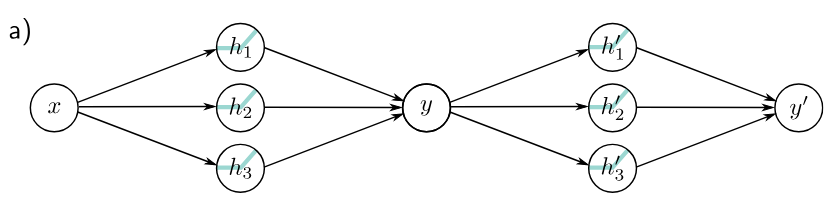
\includegraphics[scale=.42]{../assets/dl/compose.png}
    \caption{Composing neural nets}
\end{figure}

\begin{figure}[!ht]
    \centering
    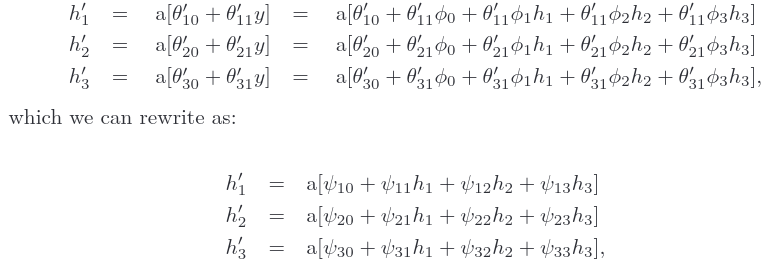
\includegraphics[scale=.47]{../assets/dl/calc.png}
    \caption{}
\end{figure}
where $y = \phi_0 + \phi_1h_1 + \phi_2h_2 + \phi_3h_3$. Here, if we compare above set of equation, we get the values of $\psi_{10} = \theta'_{10} + \theta'_{11}\phi_0$, $\psi_{11} = \theta'_{11}\phi_1$, $\psi_{12} = \theta'_{11}\phi_2$, $\psi_{13} = \theta'_{11}\phi_3$ and similarly for other parameters. The above values of $\psi_{ij}$ are the elements of first row of the outer product matrix of $ u = [\theta'_{11}, \theta'_{21}, \theta'_{31}]^\top, v = [\phi_1, \phi_2, \phi_3]^\top$.

$$ u \otimes v = \begin{bmatrix}
    \theta'_{11}\phi_1 & \theta'_{11}\phi_2 & \theta'_{11}\phi_3 \\
    \theta'_{21}\phi_1 & \theta'_{21}\phi_2 & \theta'_{21}\phi_3 \\
    \theta'_{31}\phi_1 & \theta'_{31}\phi_2 & \theta'_{31}\phi_3 \\
\end{bmatrix} $$
Hence, when we compose two neural networks the values of the parameters $\psi_{ij}$ are restricted to this outer product, while when we create a neural network with two hidden layers, we can have more values of the parameters $\psi_{ij}$ hence it can represent a broader family of functions.





\end{document}